\subsection{Diffusion NMR}
\label{subsec:poise__diffusion}

As the final example of a POISE optimisation, I demonstrate its application to \acf{dosy} experiments.\autocite{Johnson1999PNMRS}
DOSY experiments measure molecular diffusion during a delay period, $\Delta$, which is placed between two gradients, such as in the stimulated echo experiment (\cref{fig:poise_dosy_pulseq_ste}), or the bipolar pulse pair version (\cref{fig:poise_dosy_pulseq_stebpp}) which uses opposing gradients to refocus the lock signal during the sequence.
In these sequences, the first `encoding' gradient (or set thereof) imparts a spatially-dependent phase, which---in the absence of diffusion---is perfectly refocused by the second `decoding' gradient (or set thereof).
However, if diffusion is present, this refocusing is not complete, leading to signal attenuation which is described by the Stejskal--Tanner equation:
\begin{equation}
    \label{eq:stejskal_tanner_again}
    I(G) = I(0) \exp\left[-(\gamma\delta G)^2 D \Delta'\right].
\end{equation}
Here, $G$ is the amplitude of the encoding and decoding gradients, $\delta$ the duration of the gradients, and $\Delta'$ is a corrected diffusion delay.

\begin{figure}[htb]
    \centering
    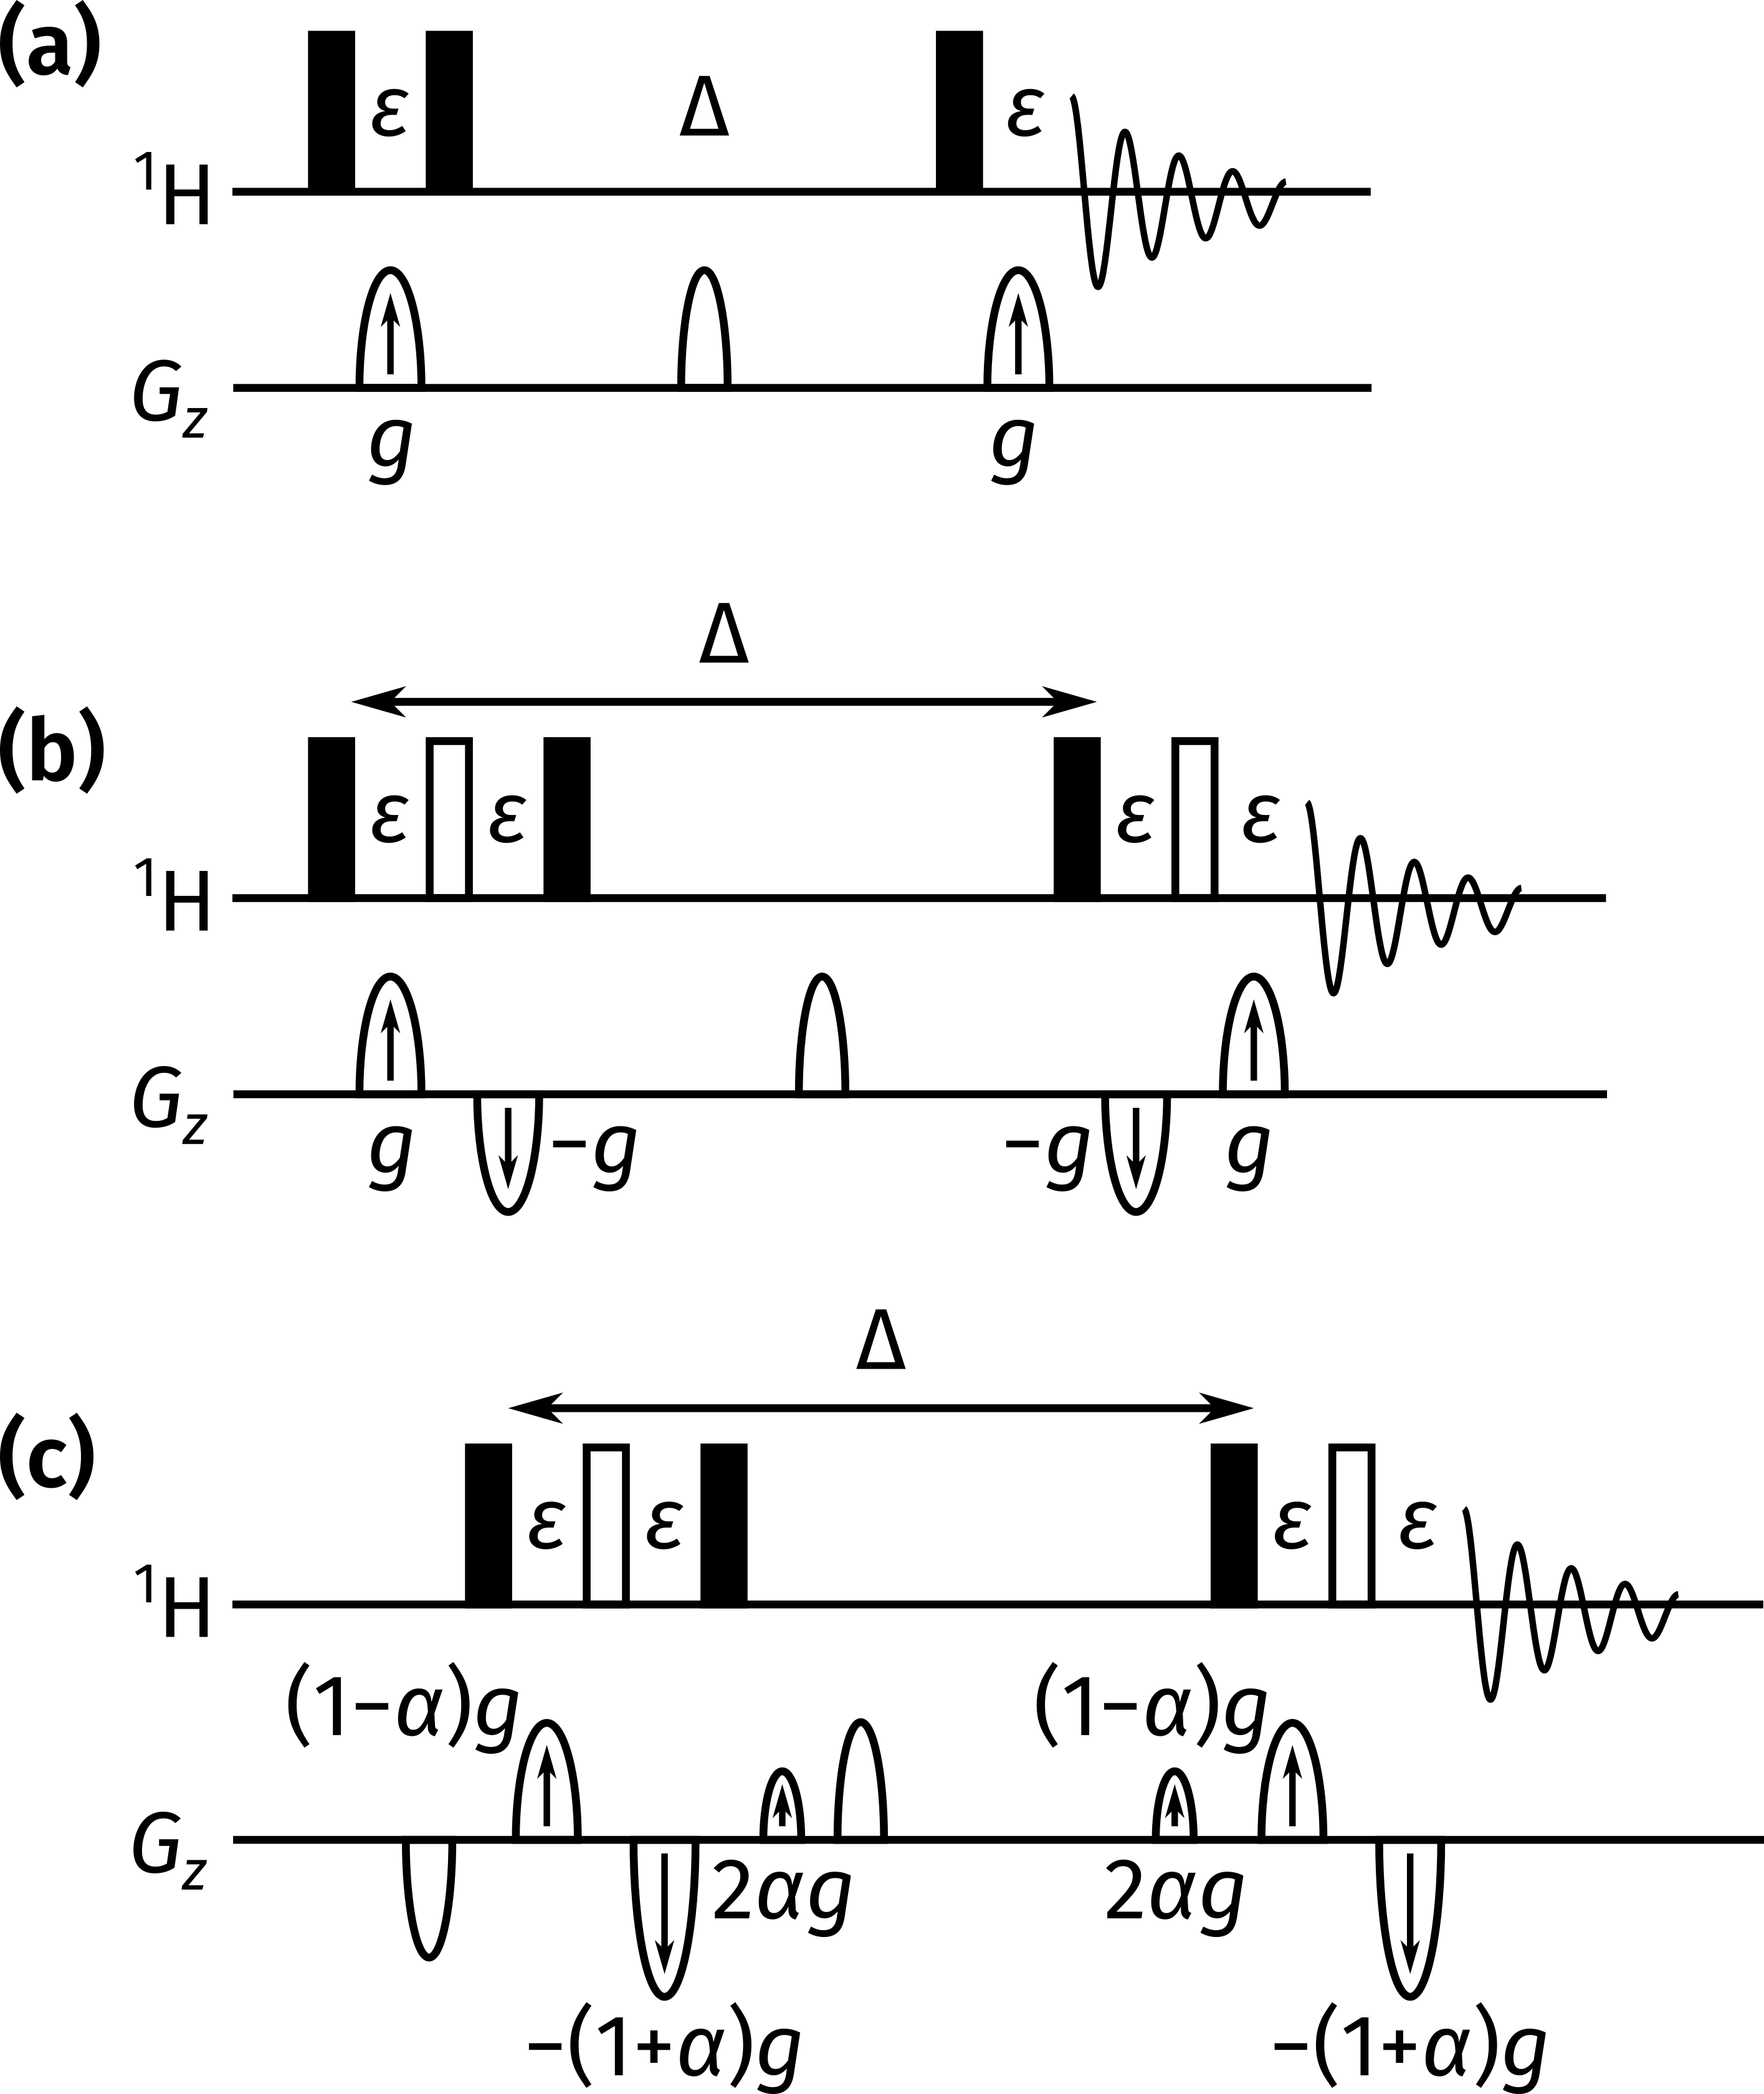
\includegraphics[]{pp/poise/dosy.png}
    {\phantomsubcaption\label{fig:poise_dosy_pulseq_ste}}
    {\phantomsubcaption\label{fig:poise_dosy_pulseq_stebpp}}
    {\phantomsubcaption\label{fig:poise_dosy_pulseq_oneshot}}
    \caption[Selection of DOSY pulse sequences]{
        \textbf{(\subref*{fig:poise_dosy_pulseq_ste})} Stimulated echo DOSY pulse sequence. The diffusion-encoding and -decoding gradients, whose amplitudes are incremented, are marked with arrows.
        \textbf{(\subref*{fig:poise_dosy_pulseq_stebpp})} Stimulated echo bipolar pulse pair DOSY pulse sequence.
        \textbf{(\subref*{fig:poise_dosy_pulseq_oneshot})} Oneshot DOSY pulse sequence.
    }
    \label{fig:poise_dosy_pulseq}
\end{figure}

In a 2D DOSY experiment, each increment is recorded with a different gradient amplitude $G$.
The value of $D$ can then be extracted through various means, most simply an exponential fitting of the measured intensities $I(G)$ for single species (or distinct species which do not overlap).
In order to minimise the uncertainty in the calculated diffusion coefficients, the parameters $\Delta$ and $\delta$, as well as the range of gradient amplitudes used (and possibly also their distribution), should be chosen in order to yield a diffusion profile of the form in \cref{fig:diffusion_sim_ok}.
Generally, the last increment (acquired using the maximum gradient strength, $G_\text{max}$ should have an attenuation of 5--35\%\footnote{Recommendations tend to vary.} when compared against the first increment (acquired with the minimum gradient amplitude, $G_\text{min}$, which may be 0).
Traditionally, this is done `by hand' by acquiring individual increments of the 2D diffusion experiment, checking the attenuation, and adjusting the parameters accordingly.\autocite{Johnson1999PNMRS,Claridge2016}

\begin{figure}[htb]
    \centering
    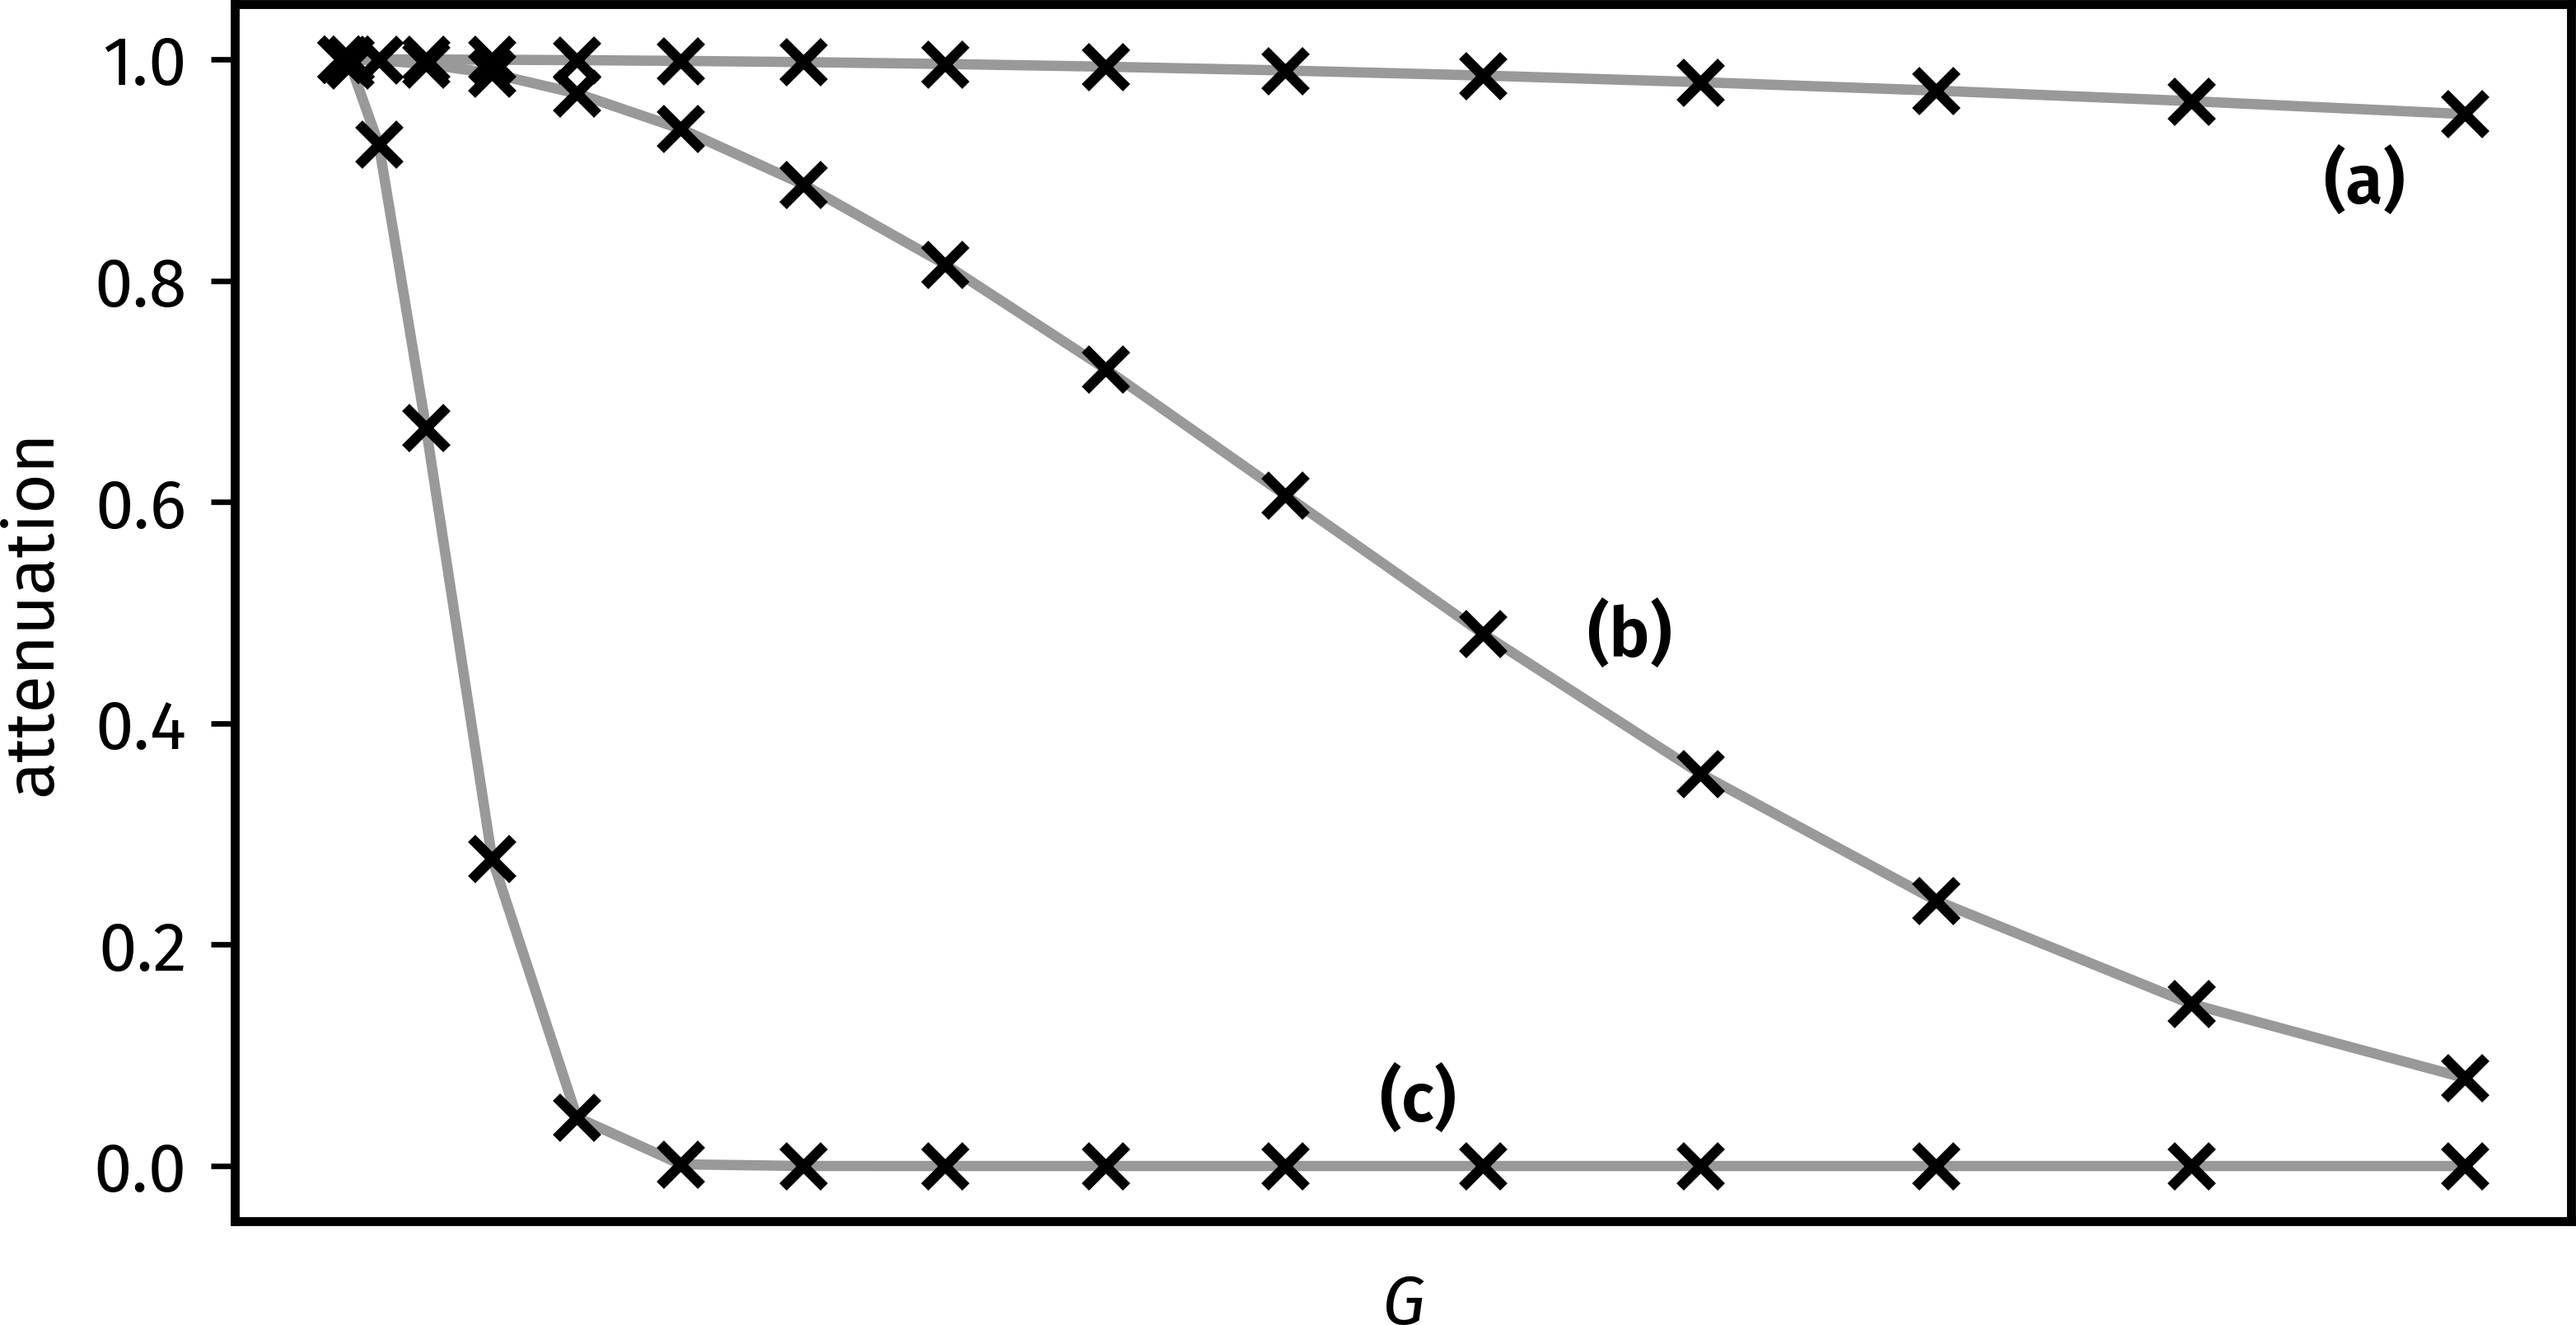
\includegraphics[]{poise/diffusion_sim.png}%
    {\phantomsubcaption\label{fig:diffusion_sim_weak}}%
    {\phantomsubcaption\label{fig:diffusion_sim_ok}}%
    {\phantomsubcaption\label{fig:diffusion_sim_strong}}%
    \caption[Simulated diffusion profiles for slow, intermediate, and rapid diffusion]{
        Simulated diffusion profiles for species with different diffusion rates.
        \textbf{(\subref*{fig:diffusion_sim_weak})} A slowly diffusing species: insufficient attenuation is observed with the given parameters, meaning that generally $\Delta$ or $\delta$ need to be increased.
        \textbf{(\subref*{fig:diffusion_sim_ok})} An `ideal' diffusion profile where attenuation is neither too little or too much.
        \textbf{(\subref*{fig:diffusion_sim_strong})} A rapidly diffusing species, for which complete attenuation is already accomplished using low gradient amplitudes. This generally suggests that $\Delta$ or $\delta$ need to be decreased, or a new gradient ramp calculated.
    }
    \label{fig:diffusion_sim}
\end{figure}

This task could of course be delegated to a computer programme such as POISE.
We \textit{could} simply tackle it head-on by optimising all of $\Delta$, $\delta$, and $G_\text{max}$ at once (assuming that $G_\text{min}$ is fixed); however, this is actually rather inefficient.
Firstly, we previously saw that multiple-parameter optimisations took a longer time than the corresponding single-parameter optimisations.
However, on top of that, it is often not even necessary to change all three parameters: the Stejskal--Tanner equation shows that the diffusion attenuation is controlled only by the overall \textit{product} $\delta^2 G_\text{max}^2 \Delta'$.
Thus, at least to a first approximation, the individual values of $\Delta$, $\delta$, and $G_\text{max}$ do not actually matter.
It makes sense to fix two of these and optimise one parameter, only changing the other two if necessary.

It should be mentioned here that obtaining \textit{accurate} values of $D$ requires careful consideration of various factors such as the exact DOSY sequence and gradient shapes used\autocite{Sinnaeve2012CMR}, peak overlap\autocite{Antalek1996JACS,Windig1997CILS,Nilsson2006AC,Nilsson2008AC,Colbourne2011JACS}, and convection\autocite{Swan2015JMR,Barbosa2016RSCA}.
This may influence the type of processing which is chosen for extraction of diffusion coefficients.
However, these issues are not our concern here: the role of POISE is only to find a good set of acquisition parameters such that the resulting data is amenable towards further processing.


\subsubsection{Optimisation setup}

The overall strategy for this `optimisation' can be briefly summarised in a flowchart (\cref{fig:dosy_flowchart}).
Note that this is \textit{not} a classic optimisation which falls nicely into the POISE workflow (\cref{fig:poise_flowchart}): thus, the entire procedure cannot simply be summarised into one POISE routine.
However, it does contain two optimisation subproblems: one to adjust $\Delta$ if necessary, and one to find $G_\text{max}$.
We can therefore create a wrapper script for the overall procedure (here called \texttt{dosy\_opt.py}, which invokes POISE to solve the two individual subproblems.
This approach is made possible by the command-line interface of POISE, which allows for the creation and execution of optimisation routines.
We also exploit the fact that during the optimisation, POISE stores the value of the cost function as the \texttt{TI} parameter in TopSpin.
This fact is often irrelevant as the value of the cost function is not often of great interest, but proves to be handy in this particular instance as it allows POISE to pass information back to the wrapper script.
Previously, we explored situations where the functionality of POISE could be extended from \textit{within}, e.g.\ by invoking different scripts in its acquisition AU programme.
In this case, we are going in the other direction, allowing POISE to be incorporated in other scripts.

\begin{figure}[htb]
    \centering
    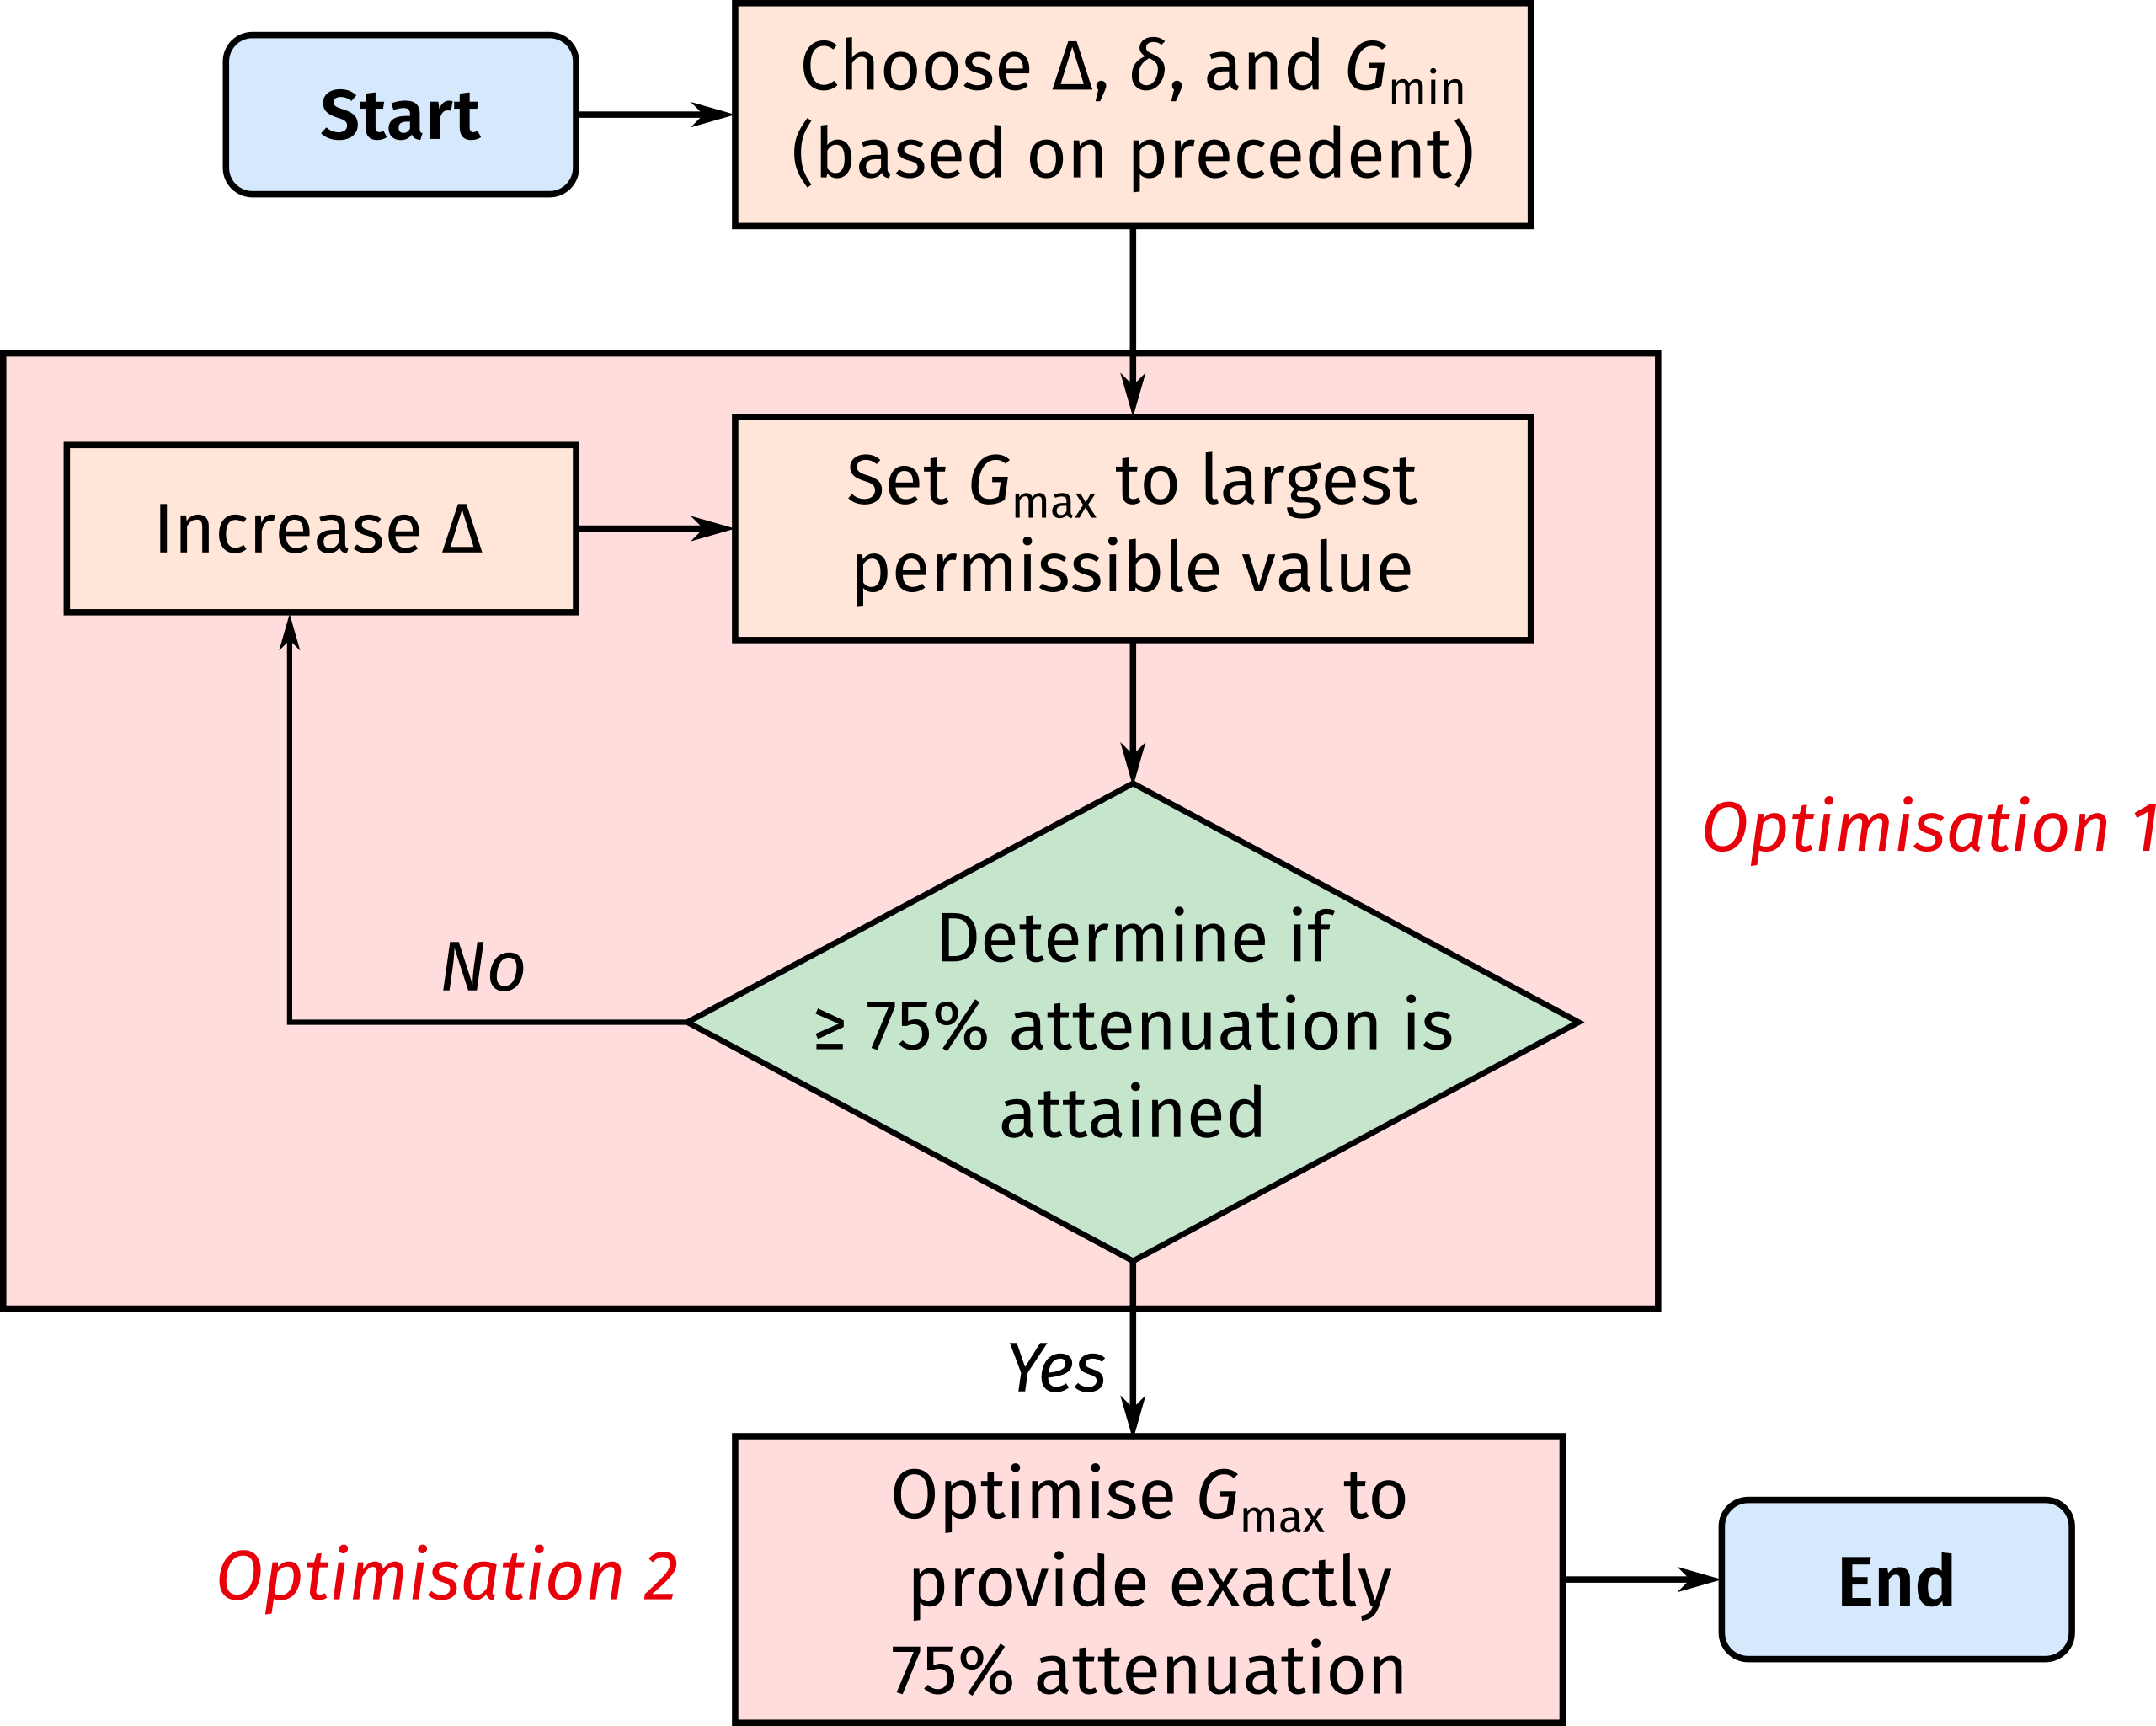
\includegraphics[]{poise/dosy_flowchart.png}%
    \caption[Flowchart for DOSY parameter optimisation]{
        Flowchart for DOSY parameter optimisation. In fact, this consists of two subproblems which can be individually solved using POISE.
    }
    \label{fig:dosy_flowchart}
\end{figure}

The DOSY optimisation procedure uses a 1D pulse programme throughout: this should essentially be a single increment of the desired 2D DOSY experiment.%
\footnote{1D versions of most DOSY variants are available in the TopSpin standard library, but can also be easily obtained by disabling the gradient incrementation in the 2D versions.}
In this work, I specifically used the Oneshot DOSY sequence\autocite{Pelta2002MRC} (\cref{fig:poise_dosy_pulseq_oneshot}): this sequence has the advantage of not requiring onerously long phase cycles, which would otherwise lead to very long FEs and optimisations.\footnote{However, using \textit{too few} scans leads to inaccuracies in the diffusion coefficients.\autocite{Pelta2002MRC} I chose to use 4 scans per FE here.}
In principle, though, the optimisation can be run with any DOSY variant, including convection-compensated sequences\autocite{Jerschow1997JMR,Sorland2000JMR,Nilsson2005JMR}: the \texttt{dosy\_opt.py} wrapper script is sufficiently general that only minor modifications are needed to use it with other DOSY sequences.

The first optimisation subproblem is the determination of an appropriate diffusion delay $\Delta$.
Since larger diffusion delays lead to a greater loss of signal through $T_1$ relaxation, as well as more convection\autocite{Swan2015JMR}, $\Delta$ should always be kept as short as possible.%
\footnote{In hindsight, it would likely have been better to increase $\delta$ instead: this would also have a larger effect as the attenuation depends quadratically on $\delta$ but only linearly on $\Delta$. Care must be taken to not increase $\delta$ beyond what the spectrometer can tolerate, though.}
Since the procedure in \cref{fig:dosy_flowchart} only \textit{increases} $\Delta$, the wrapper script should always be started with the smallest value of $\Delta$ which is sensible for the sample under study: in the present case, I used an initial value of \qty{50}{\ms}.
The next step is to determine whether using the full range of available gradient amplitudes leads to sufficient attenuation (which I defined to be 75\%), relative to the first increment of the DOSY acquired using $G_\text{min}$.
This involves setting $G_\text{max}$ to the largest permissible value (for the Oneshot sequence, this is 80\%), then calculating a cost function $f_\text{dosy,aux}$:
\begin{equation}
    \label{eq:dosy_aux_cf}
    f_\text{dosy,aux} = \frac{\sum_i S_i(G_\text{max})}{\sum_i S_i(G_\text{min})} - 0.25.
\end{equation}
In the fraction, the numerator represents an integral over some region of the spectrum acquired with $G_\text{max}$, and the denominator an integral over the same region for the spectrum acquired with $G_\text{min}$.
If the attenuation is sufficient, then $f_\text{dosy,aux}$ will be negative.

In order for the wrapper script to monitor this cost function, POISE is instructed to perform an `optimisation' with only one function evaluation, using the \texttt{-\phantom{}-maxfev 1} flag: essentially, POISE is being used here purely as a way of evaluating the cost function $f_\text{dosy,aux}$.%
\footnote{Of course, this cost function evaluation could just be done in the wrapper script itself. In fact, it would likely be simpler to do so. But there is one clear benefit of doing it in this rather circuitous route: POISE allows the user to write cost functions in Python 3.}
At each point, POISE stores the value of $f_\text{dosy,aux}$ in the \texttt{TI} parameter, and returns control to the wrapper script so that it can check this value.
If the value of $f_\text{dosy,aux}$ is negative, then the wrapper script moves on to the next subproblem.
However, if it is still positive, then there is no way the desired attenuation can be accomplished using the gradient strengths available.
Thus, $\Delta$ is increased by a fixed amount (\qty{50}{\ms} in this case), and the sub-optimisation step repeated.\footnote{If sample spinning is used, then this incrementation of $\Delta$ needs to be chosen carefully, as the diffusion delay should always correspond to an integral number of rotations.}

Once a suitable value of $\Delta$ has been found, the script then searches for the correct value of $G_\text{max}$ in order to provide \textit{exactly} the `correct' amount of attenuation (in this case, 75\%).
This is done through a conventional POISE optimisation, where the cost function is
\begin{equation}
    \label{eq:dosy_cf}
    f_\text{dosy} = |f_\text{dosy,aux}| = \left| \frac{\sum_i S_i(G_\text{max})}{\sum_i S_i(G_\text{min})} - 0.25 \right|.
\end{equation}
The absolute value here makes sure that the optimisation converges to the value of $G_\text{max}$ which gives \textit{precisely} a 75\% attenuation, no more, and no less.
At this point, the wrapper script reports the appropriate values of $\Delta$ and $G_\text{max}$, and then exits; these values can then be used to set up a DOSY experiment (e.g.\ using the \texttt{dosy} TopSpin AU programme).

Before presenting some results, it is worth contemplating what would happen if the sample under study contained a mixture of different molecules, as would often be the case in DOSY experiments.
Assuming that the integrals $\sum_i S_i$ are taken over the entire spectrum, the parameters thus obtained would then be `compromise values' which are weighted more heavily towards the major component(s) in the sample.
This spectral region being evaluated can be changed by the user (via the \texttt{dpl} command), but that relies on some knowledge of the sample being studied.
Thus, in this case, our best hope is really that the `compromise' parameters obtained are \textit{good enough} for all the components in the mixture.
Obviously, this can hardly be guaranteed, and the larger the difference in the diffusion coefficients of the constituent species, the more prone this approach is to failing.

In my defence, any script which seeks to optimise DOSY parameters must account for the presence of mixtures in some way, for example by identifying rapidly- and slowly-diffusing species.
This is therefore not truly an issue with POISE \textit{per se}, but rather with the approach taken in the wrapper script.
(For example, if the wrapper script can identify distinct resonances which have different attenuation profiles, then POISE could be used to perform individual optimisations on each of these.)
Nevertheless, for this reason, I refrain from claiming that the work in this section constitutes a \textit{full} method for automating DOSY.%
\footnote{Doing such an endeavour proper justice would anyway have required rather more time in my DPhil and more space in this thesis.}
I am more comfortable labelling this as a demonstration of how POISE can be integrated into larger procedures---for example, in the setup of single-component DOSY experiments.


\subsubsection{Optimisation results}

The DOSY optimisation procedure described above was tested on the sample of andrographolide (in DMSO-$d_6$).
Despite this being a single-component sample, it does at least have some mildly interesting behaviour, in that the exchangeable \ch{OH} protons have a larger apparent diffusion coefficient compared to the \ch{CH} protons.

As described previously, the procedure was initialised with a value of $\Delta = \qty{50}{\ms}$.
The gradient duration $\delta$, which is not modified, was set to \qty{2}{\ms}.
The first sub-optimisation always increased the value of the diffusion delay by one step to \qty{100}{\ms}.
Since this part only uses one function evaluation in POISE, the optimisation algorithm used does not actually matter.
However, the algorithm does matter for the second sub-optimisation (which searches for the best value of $G_\text{max}$).
This part was therefore performed five times per algorithm, in line with previous optimisations in this chapter (\cref{tbl:poise_dosy_opt2}).

\begin{table}[htb]
    \hbadness=10000
    \centering
    \begin{tabular}{ccccc}
        \toprule
        Entry & Algorithm & Optimum found (\%) & FEs  & Time taken (\unit{\s}) \\
        \midrule
        1     & NM        & 75.00              & 9    & 195--197             \\
        2     & MDS       & 75.00              & 9    & 196--197             \\
        3     & BOBYQA    & 75.00--75.60       & 8--9 & 175--197             \\
        \bottomrule
    \end{tabular}
    \caption[DOSY maximum gradient amplitude sub-optimisations]{
        Results of maximum gradient amplitude sub-optimisations for DOSY parameter setup.
        The POISE routine used here is: \mintinline[breaklines]{json}{{"name": "dosy", "pars": ["gpz1"], "lb": [20.0], "ub": [80.0], "init": [50.0], "tol": [2.0], "cf": "dosy", "au": "poise_1d"}}.
        \datacode{6A-200823}
    }
    \label{tbl:poise_dosy_opt2}
\end{table}

In this case, all three algorithms converged to the same result of $75\%$.
The full Oneshot DOSY spectrum was then acquired using these parameters of $\Delta = \qty{100}{\ms}$, $\delta = \qty{2}{\ms}$, and $G_\text{max} = 75\%$ (nominally \qty{49.3}{\gauss\per\cm} on the spectrometer used here, see \cref{tbl:spectrometers}).
The overall time taken was approximately five minutes: two for the first sub-optimisation to find $\Delta$, and three for the second sub-optimisation (as shown in \cref{tbl:poise_dosy_opt2}).
This figure may of course be larger depending on the number of scans used (here I used \texttt{DS=2} and \texttt{NS=4}), as well as the number of iterations required in the first sub-optimisation.

The resulting attenuation profiles for one \ch{CH} and one \ch{OH} peak are shown in \cref{fig:poise_diffusion_profiles}.
The apparently more slowly-diffusing \ch{CH} peak is attenuated to 28\% of its original intensity, whereas the exchanging \ch{OH} peak is attenuated to 20\%.
This is certainly a case where the `different components' have diffusion coefficients which are not too dissimilar, allowing reasonable results to be obtained.
Gaussian fitting using the modified Stejskal--Tanner equation
\begin{equation}
    \label{eq:stejskal_tanner_oneshot}
    I(G) = I(0) \exp\left\{-(\gamma\delta G)^2 D \left[\Delta - \frac{\delta(5 - 3\alpha^2)}{16} - \frac{\tau(1-\alpha^2)}{2}\right]\right\}
\end{equation}
yielded \textit{apparent} diffusion coefficients of \qty{7.411(13)e-9}{\m\squared\per\s} for the \ch{CH} peak and \qty{9.369(49)e-9}{\m\squared\per\s} for the \ch{OH} peak.
(The equation was obtained from the pulse programme provided on the University of Manchester website; here $\tau$ represents the time between the midpoints of each gradient within the bipolar pulse pair, and $\alpha$ the gradient imbalance factor as shown in \cref{fig:poise_dosy_pulseq_oneshot}.)

\begin{figure}[htb]
    \centering
    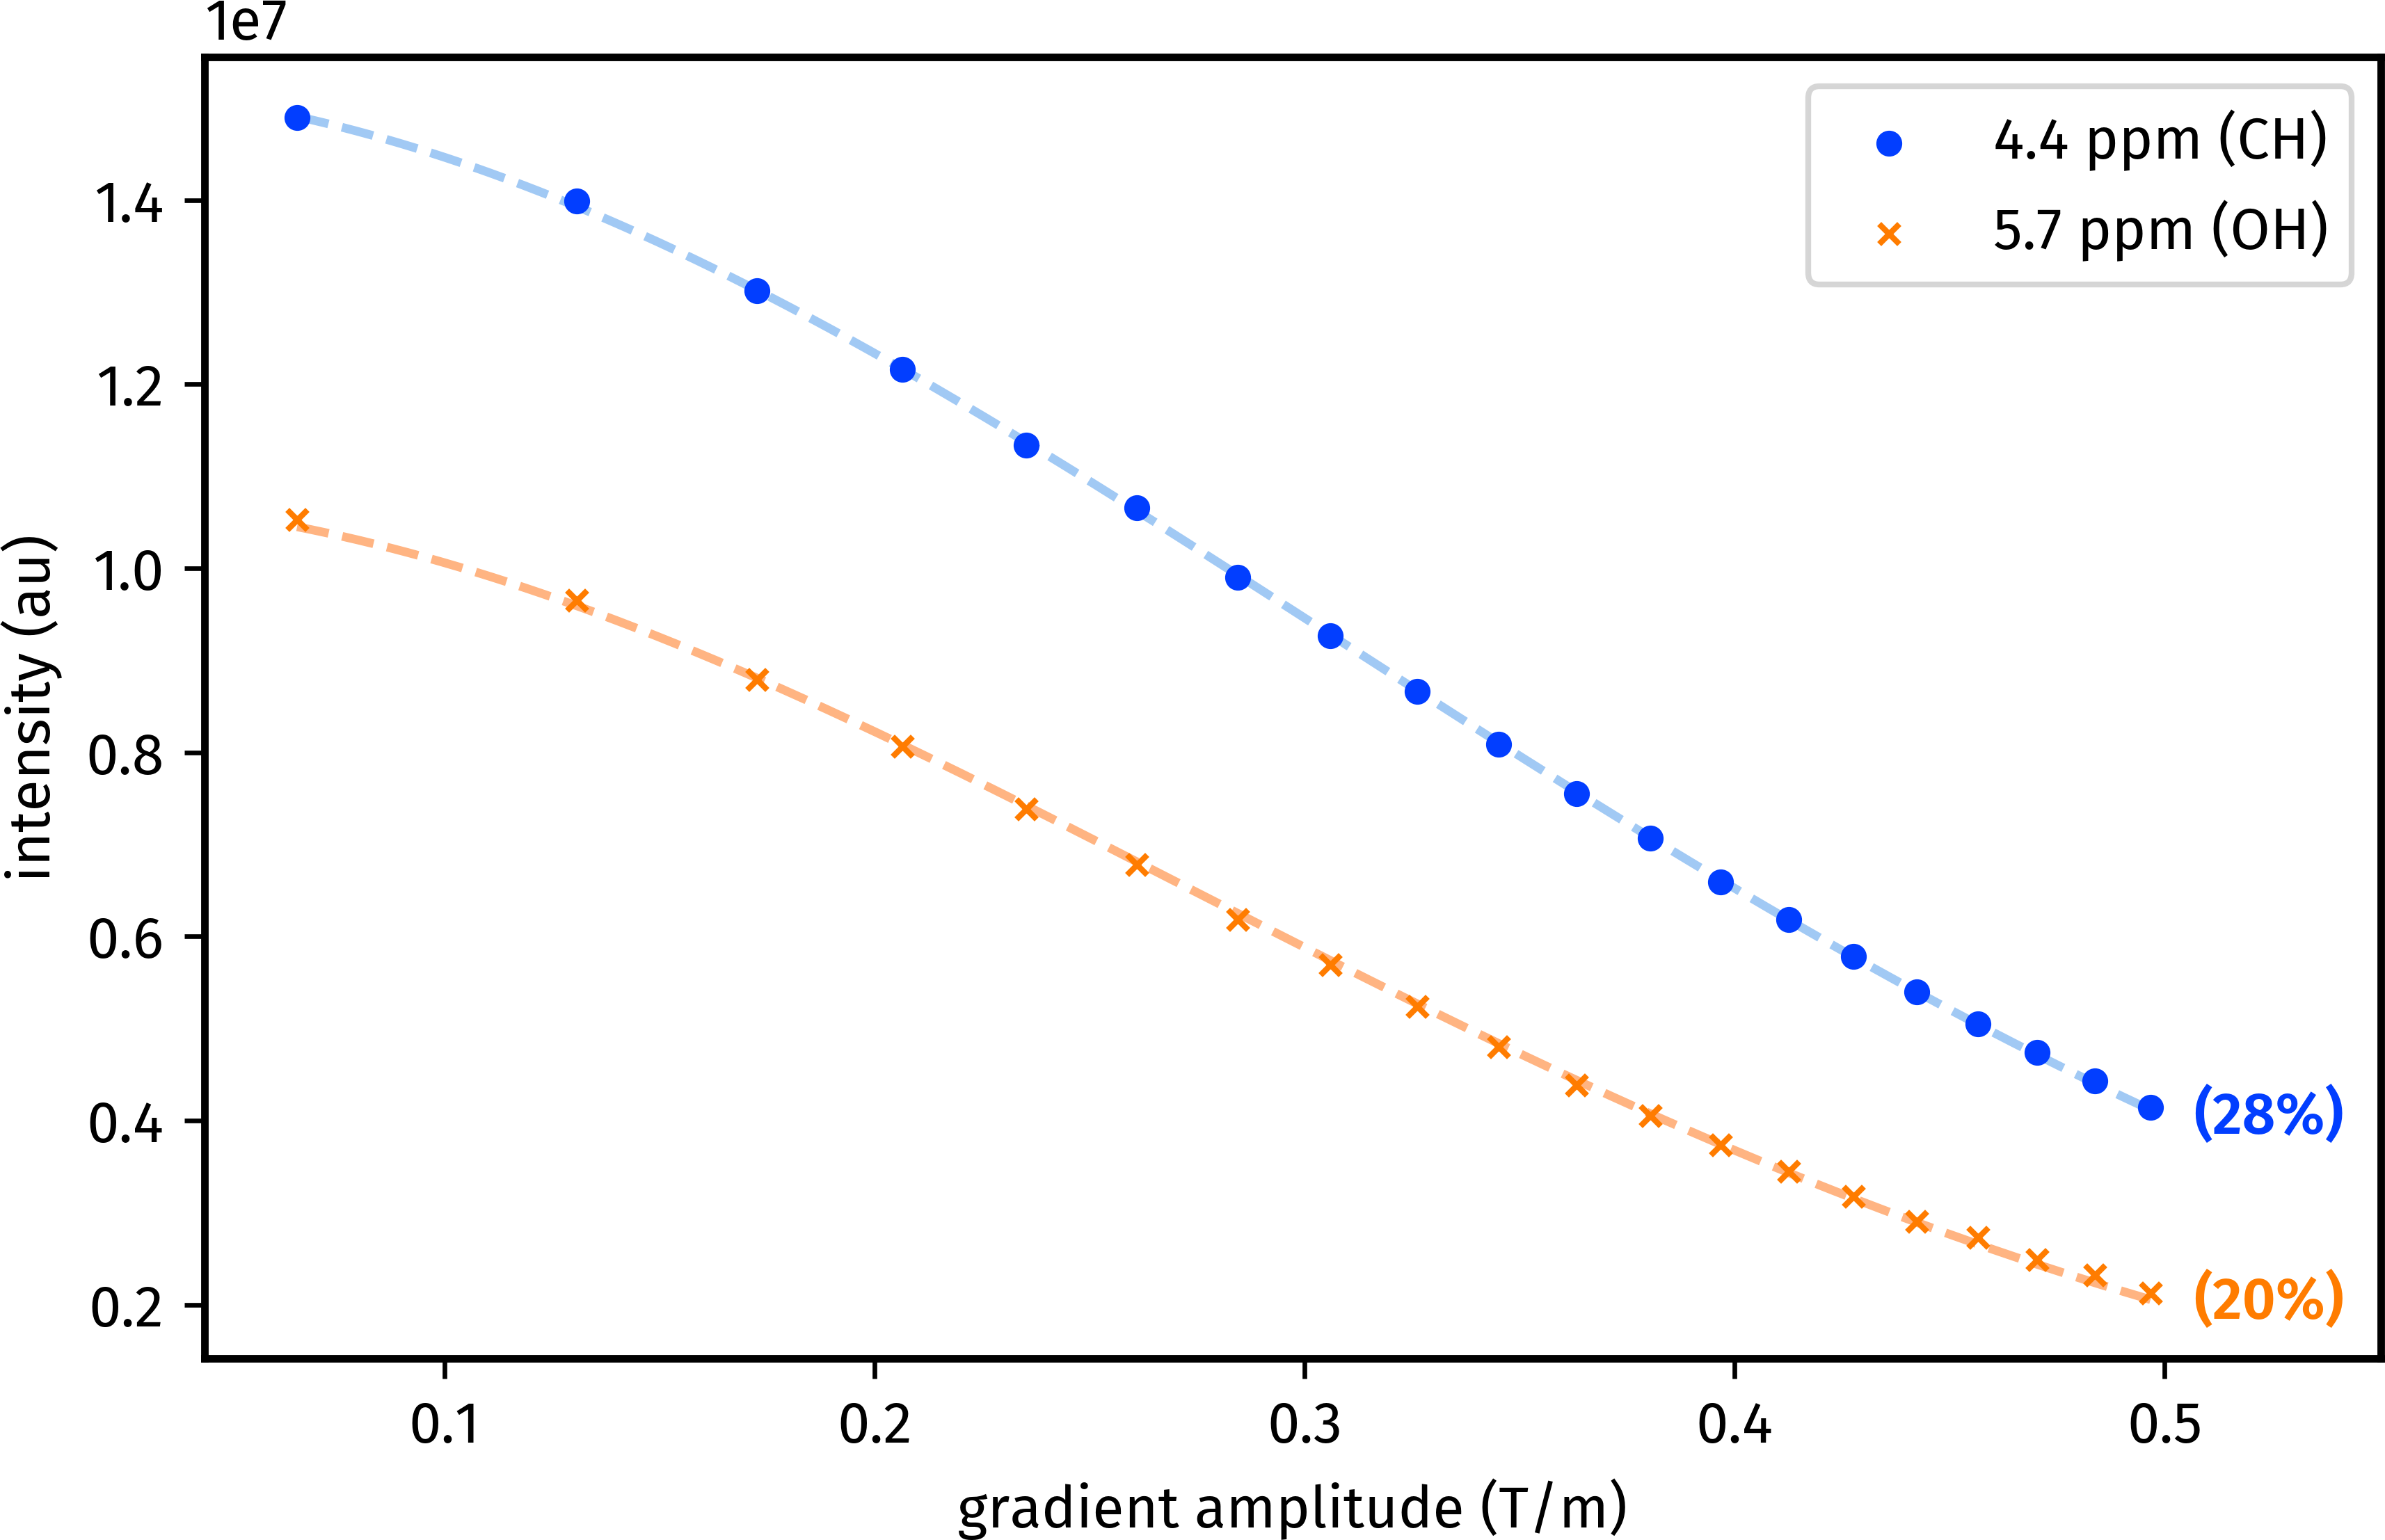
\includegraphics[]{poise/dosy_profiles.png}%
    \caption[Diffusion profiles of \ch{CH} and \ch{OH} peaks after optimisation of DOSY parameters]{
        Diffusion profiles obtained using a Oneshot experiment for a \ch{CH} peak (blue, circles) and an \ch{OH} peak (orange, crosses) in andrographolide.
        The dashed lines represent the Gaussian curves obtained through non-linear least-squares fitting (\texttt{scipy.optimize.curve\_fit}).
        \datacode{6A-200823}
    }
    \label{fig:poise_diffusion_profiles}
\end{figure}




\subsubsection{Simultaneous optimisation of $\symbf{\Delta}$ and $\symbfit{G}_\text{max}$}

It is possible---albeit inefficient, as previously mentioned---to dispense with the wrapper script entirely and perform a single optimisation of both $\Delta$ and $G_\text{max}$.
In order to ensure that $\Delta$ is not increased too much, we must add a penalty term to the cost function:
\begin{equation}
    \label{eq:dosy_2p_cf}
    f_\text{dosy,2p} = f_\text{dosy} + (\Delta / \unit{\s}) = \left| \frac{\sum_i S_i(G_\text{max})}{\sum_i S_i(G_\text{min})} - 0.25 \right| + (\Delta / \unit{\s})
\end{equation}
(where `2p' stands for two-parameter).
One significant drawback of this is that the reference spectrum $\symbf{S}(G_\text{min})$ must be reacquired every time $\Delta$ is changed: so, each FE requires twice as long as before.
For example, using the NM algorithm, the optimisation converged to $\Delta = \qty{91.6}{\ms}$ and $G_\text{max} = 79.3\%$.
Although this result is quite similar to what we had obtained before, the optimisation took over 26 minutes, over five times longer than previously.
I therefore opted not to perform the full 15 optimisations.

Curiously, BOBYQA did not work as well with this cost function: in the two times I tested it, BOBYQA converged to an `optimum' of $\Delta = \qty{225}{\ms}$ and $G_\text{max} = 50\%$.
This did yield the expected 75\% attenuation in the spectrum, but $\Delta$ is clearly rather longer than we would like it to be.
Furthermore, because of the penalty term, the value of the cost function at this point (0.229) was far larger than the corresponding optimum found using the NM algorithm (0.095).
It is likely that some of the trust-region optimisation parameters must be tweaked to make this work properly, but I did not spend any further time investigating this.
